% Do not forget to include Introduction
%---------------------------------------------------------------
%\chapter{Introduction}
% uncomment the following line to create an unnumbered chapter
\chapter*{Introduction}\addcontentsline{toc}{chapter}{Introduction}\markboth{Introduction}{Introduction}
%---------------------------------------------------------------
\setcounter{page}{1}

% The following environment can be used as a mini-introduction for a chapter. Use that any way it pleases you (or comment it out). It can contain, for instance, a summary of the chapter. Or, there can be a quotation.
%\begin{chapterabstract}
%\end{chapterabstract}

Modern high-performance network devices are usually proprietary systems that combine custom hardware, specialized operating systems, and tightly coupled software. 
While these solutions offer high throughput and reliability, they are typically expensive, inflexible, and slower to evolve due to their closed design and development model.
Vector Packet Processing (VPP) is a high-performance network stack that operates at layers 2 to 4 of the ISO/OSI model. 
It was originally developed by Cisco Systems, Inc. (which is a world leader in networking) and open-sourced in 2016 under the Fast Data Project (FD.io), that is part of the Linux Foundation.
VPP brings the ability to perform efficient, high-speed packet processing on common off-the-shelf (COTS) hardware, across a wide range of platforms and operating systems.
Its open and flexible architecture opens the door to a new class of network applications that can be deployed and scaled more easily than traditional hardware appliances. 
In this way, VPP could represent a shift in the traditionally conservative networking world, echoing the "Mainframe to PC" revolution, 
where general-purpose systems replaced proprietary platforms, enabling broader innovation and accessibility.

Since VPP was open-sourced only recently, it has not yet been widely adopted by the market, and there are only a limited number of academic studies on the subject. As a result, this area remains underexplored. 
This thesis aims to contribute to this field by evaluating VPP's\footnote{The abbreviation VPP is also commonly used in academic literature to refer to a Virtual Power Plant.} performance, 
with a particular focus on its electricity consumption. 
The findings could provide valuable insights for the industry and guide future research, especially in light of the increasing importance of energy efficiency, 
as highlighted in recent forecasts by ČEPS a.s. regarding the future of energy resources in the Czech Republic.

With the development of AI and the growing demand for high-resolution streaming services, it is highly likely that the demand for internet bandwidth will continue to rise. 
This will result in an increased need for network equipment capable of processing larger volumes of data more efficiently. 
Therefore, it is crucial to explore technologies like VPP that are capable to handle this growing demand and to explore their energy efficiency.

This thesis is divided into two parts: Theoretical and Practical. 
The Theoretical part presents the traditional approach to networking and packet processing, as well as an overview of how VPP is designed and the principles on which it operates. Additionally, it introduces the testing scenarios used. 
The Practical part describes the testing infrastructure, presents the results of various measurements, and provides an analysis of the findings.

%---------------------------------------------------------------
\chapter{Theoretical part}
%---------------------------------------------------------------

%---------------------------------------------------------------
\section{"Vector Packet Processing (VPP) and Its Operating Principles}
%---------------------------------------------------------------
\begin{chapterabstract}
This section describes the fundamental principles behind the Vector Packet Processing (VPP) technology, which aims to enable efficient and high-performance network packet processing. 
VPP is built on modern programming and architectural principles that allow maximum utilization of contemporary hardware, particularly in parallel processing and memory access optimization.
\end{chapterabstract}

The section begins with a brief description of traditional network traffic processing methods used by operating systems and their limitations in terms of performance and scalability. 
Following that, the architecture of VPP is explored in detail, explaining how packets are processed in vectors, the use of a node graph, 
and the various techniques that contribute to its high efficiency—such as I/O and compute batching, zero-copy methods, and lock-free multi-threading. 
The purpose of this section is to provide a theoretical foundation for understanding how VPP operates.

\subsection{Traditional network traffic processing}
A \textit{network packet} is a basic unit of data transmitted over a network. It consists of a \textit{header}, which includes control information such as source and destination IP addresses, 
and a \textit{payload}, which carries the actual user data. 
Packets are routed independently through the network and reassembled at the destination. 
This structure allows efficient and reliable communication, even over complex or unreliable network paths.

Currently, packet processing works as follows: a packet arrives at the network card, which then
issues a system call (syscall) to the operating system for packet processing. The microprocessor
must save the currently executing instruction, perform a context switch, locate the appropriate
service routine in the interrupt vector table, and handle the packet processing. Once completed, it
must restore the saved instruction, perform another context switch, and return to processing the
interrupted program.

This system for operating peripherals was designed under the assumption that the peripherals
would not request interrupts continuously, which is not the case with network devices that need
to process large volumes of data split into small parts. 
This method requires the microprocessor to execute a significant
number of instructions not directly related to packet processing. 
Chase et al. \cite{gallatin1999trapeze} discovered \footnote{kap. 3.3 obr. 6} that if MTU is 1500 bytes, then interrupt handling accounts for 20\% - 25\% of receiver packet-processing overhead.
Another disadvantage of tradidtional packet processing is the inefficient handling of cache memory; the processing of the packets one by one in response to
interrupts leads to frequent cache misses in both cache \& inctruction caches.\footnote{kap. 4.2}\cite{cox2000profiling} 

%-----------------------------------------------------
\subsection{An Introduction to VPP}

Vector Packet Processing (VPP) is a multi-platform network stack that operates at layers 2-4 of the ISO/OSI model and is developed by the FD.io project. 
It consists of a set of forwarding vertices arranged in an oriented graph and auxiliary software and provides out-of-the-box switch/router functionality.
Unlike traditional network stacks, which run in the kernel, VPP operates in user space.

In a traditional approach, packets are processed one by one. In contrast, VPP reads the largest available number of packets called vector from the network interface card (NIC) 
and processes the entire vector through a VPP node-graph one node at a time. Each node in this graph handles a specific part of the packet processing.
This approach reduces cache misses and spreads fixed overhead costs across multiple packets, lowering the average processing cost per packet. 
Additionally, it allows VPP to take advantage of multiple cores, enabling parallel processing, which significantly improves overall performance.

Vector Packet Processing (VPP) runs on common off-the-shelf hardware (COTS), ensuring its broad compatibility and flexibility for deployment. 
It supports various architectures such as x86, ARM, and Power, and can be deployed on both standard servers and embedded devices. 
The design of VPP is agnostic to hardware, kernel, and deployment platform, meaning it can operate across a wide range of systems, including bare metal servers, virtual machines (VMs), and containers. 
This approach allows VPP to be deployed on widely available infrastructure without the need for specialized hardware.\cite{fdio_what_is_vpp}

\subsection{Techniques used in VPP}

TBD
DOPAST !!! Low-level code optimization technique

According to Linguaglossa et al.\cite{LINGUAGLOSSA} VPP uses theese kernel-bypass techniques:

\begin{itemize}
  \item \textbf{Lock-Free Multi-Threading (LFMT)}
is a programming technique that leverages modern multi-core CPUs to increase system performance. In network applications, parallelism is achieved by running multiple threads in the same time. 
Ideally, the more threads are used, the better the system performance but only up to a saturation point beyond which additional threads bring no gainns. 
However, to reach this ideal performance, traditional synchronization mechanisms such as mutexes and semaphores must be avoided, as they introduce delays due to thread contention. 
Instead, lock-free architectures have to be used, allowing threads to operate independently without blocking each other. 
In the context of VPP this approach is enabled by hardware features like multi-queue NICs, 
which allow each thread to handle a distinct subset of traffic, ensuring efficient and parallel processing.

  \item \textbf{I/O batching (IOB)}
is a key technique used in VPP. 
Instead of raising an interrupt for every incoming packet, the network interface card (NIC) collects multiple packets into a buffer and triggers an interrupt only when the buffer is full. 
This reduces the overhead caused by frequent context switching and interrupt handling. 
VPP typically uses poll-mode drivers, which collect packets in batches without relying on interrupts. 
Moreover, the batching technique is applied system-wide in VPP. This approach maximizes CPU efficiency, improves cache usage, and delivers stable, high-throughput performance even under heavy load.

  \item \textbf{Compute batching (CB)} 
is a technique that extends I/O batching to the processing phase itself. 
Instead of processing one packet at a time, network functions are designed to operate on entire batches of packets. 
This approach minimizes overhead from function calls (such as context switches and stack setup) and improves instruction cache efficiency. 
When a batch of packets enters a processing function, only the first packet might cause an instruction cache miss, while the rest benefit from already-warmed cache.
Additionally it is possible to take advatage of instruction-level parallelism.
  
  \item \textbf{Receive-Side Scaling (RSS)}
is a hardware-based technique used by modern NICs to distribute incoming packets across multiple RX queues. 
This enables parallel packet processing by allowing each queue to be handled by a separate thread, improving scalability and throughput. 
Packet assignment is typically done using a hash function over packet header fields (e.g., the 5-tuple). 

  \item \textbf{Zero-Copy (Z-C)} 
is a technique used to eliminate unnecessary memory copying during packet processing. 
Instead of copying incoming packets from the network interface card (NIC) to a separate buffer via system calls, 
the NIC writes packets directly into a pre-allocated memory region that is shared with the user-space application via Direct Memory Access (DMA). 
This allows the application to access packet data without invoking system calls or duplicating memory, significantly reducing CPU overhead. 

  \item \textbf {Cache Coherence and Locality (CC\&L)} are critical factors in the performance of modern software-based packet processing systems. 
In current COTS architectures, memory access has become a major bottleneck, which is mitigated by a multi-level cache hierarchy.
Minimizing cache misses and maintaining data locality during packet processing is essential for achieving high performance and low latency.

  \item \textbf {Low-Level Parallelism (LLP)} 
refers to the ability to exploit the internal micro-architecture of modern CPUs, including multi-stage pipelines, arithmetic-logical units (ALUs), and branch predictors that help maintain pipeline efficiency. 
Well-optimized code can keep these pipelines full and execute multiple instructions per clock cycle, increasing overall throughput. 
Performance can be further improved by giving hints to the compiler -- such as indicating the likely outcome of conditional branches -- to reduce pipeline stalls. 
Vectorized packet processing and specific coding practices can take full advantage of these hardware features and VPP was specifically designed to taky advantage of LLP.

\end{itemize}

\subsection{VPP Processing Graph and Graph nodes}
At the core of VPP (Vector Packet Processing) lies the Packet Processing Graph, a directed graph composed of relatively small, modular \& loosely coupled nodes. 
Each node is designed to perform a specific task and there are 3 types of them: \textit{process}, \textit{input} \& \textit{internal}. 
Process nodes do not participate in the packet forwarding graph; instead, they handle timers, events, and other background tasks within the VPP runtime.
Input nodes are used for input of data and internal nodes are used for vector processing. Internal nodes also serves as output nodes. 
When a vector of packets is prepared by input node, it is then pushed through the internal nodes. 
During processing, the vector may be split if the batch contains packets of different protocols or types, as they may need to follow different paths through the graph
When the original vector is completely processed, the process repeats.
Illustration of this Processing Graph is shown in fig. \ref{fig:processing-graph}.

\begin{figure}[!htbp]
    \centering
    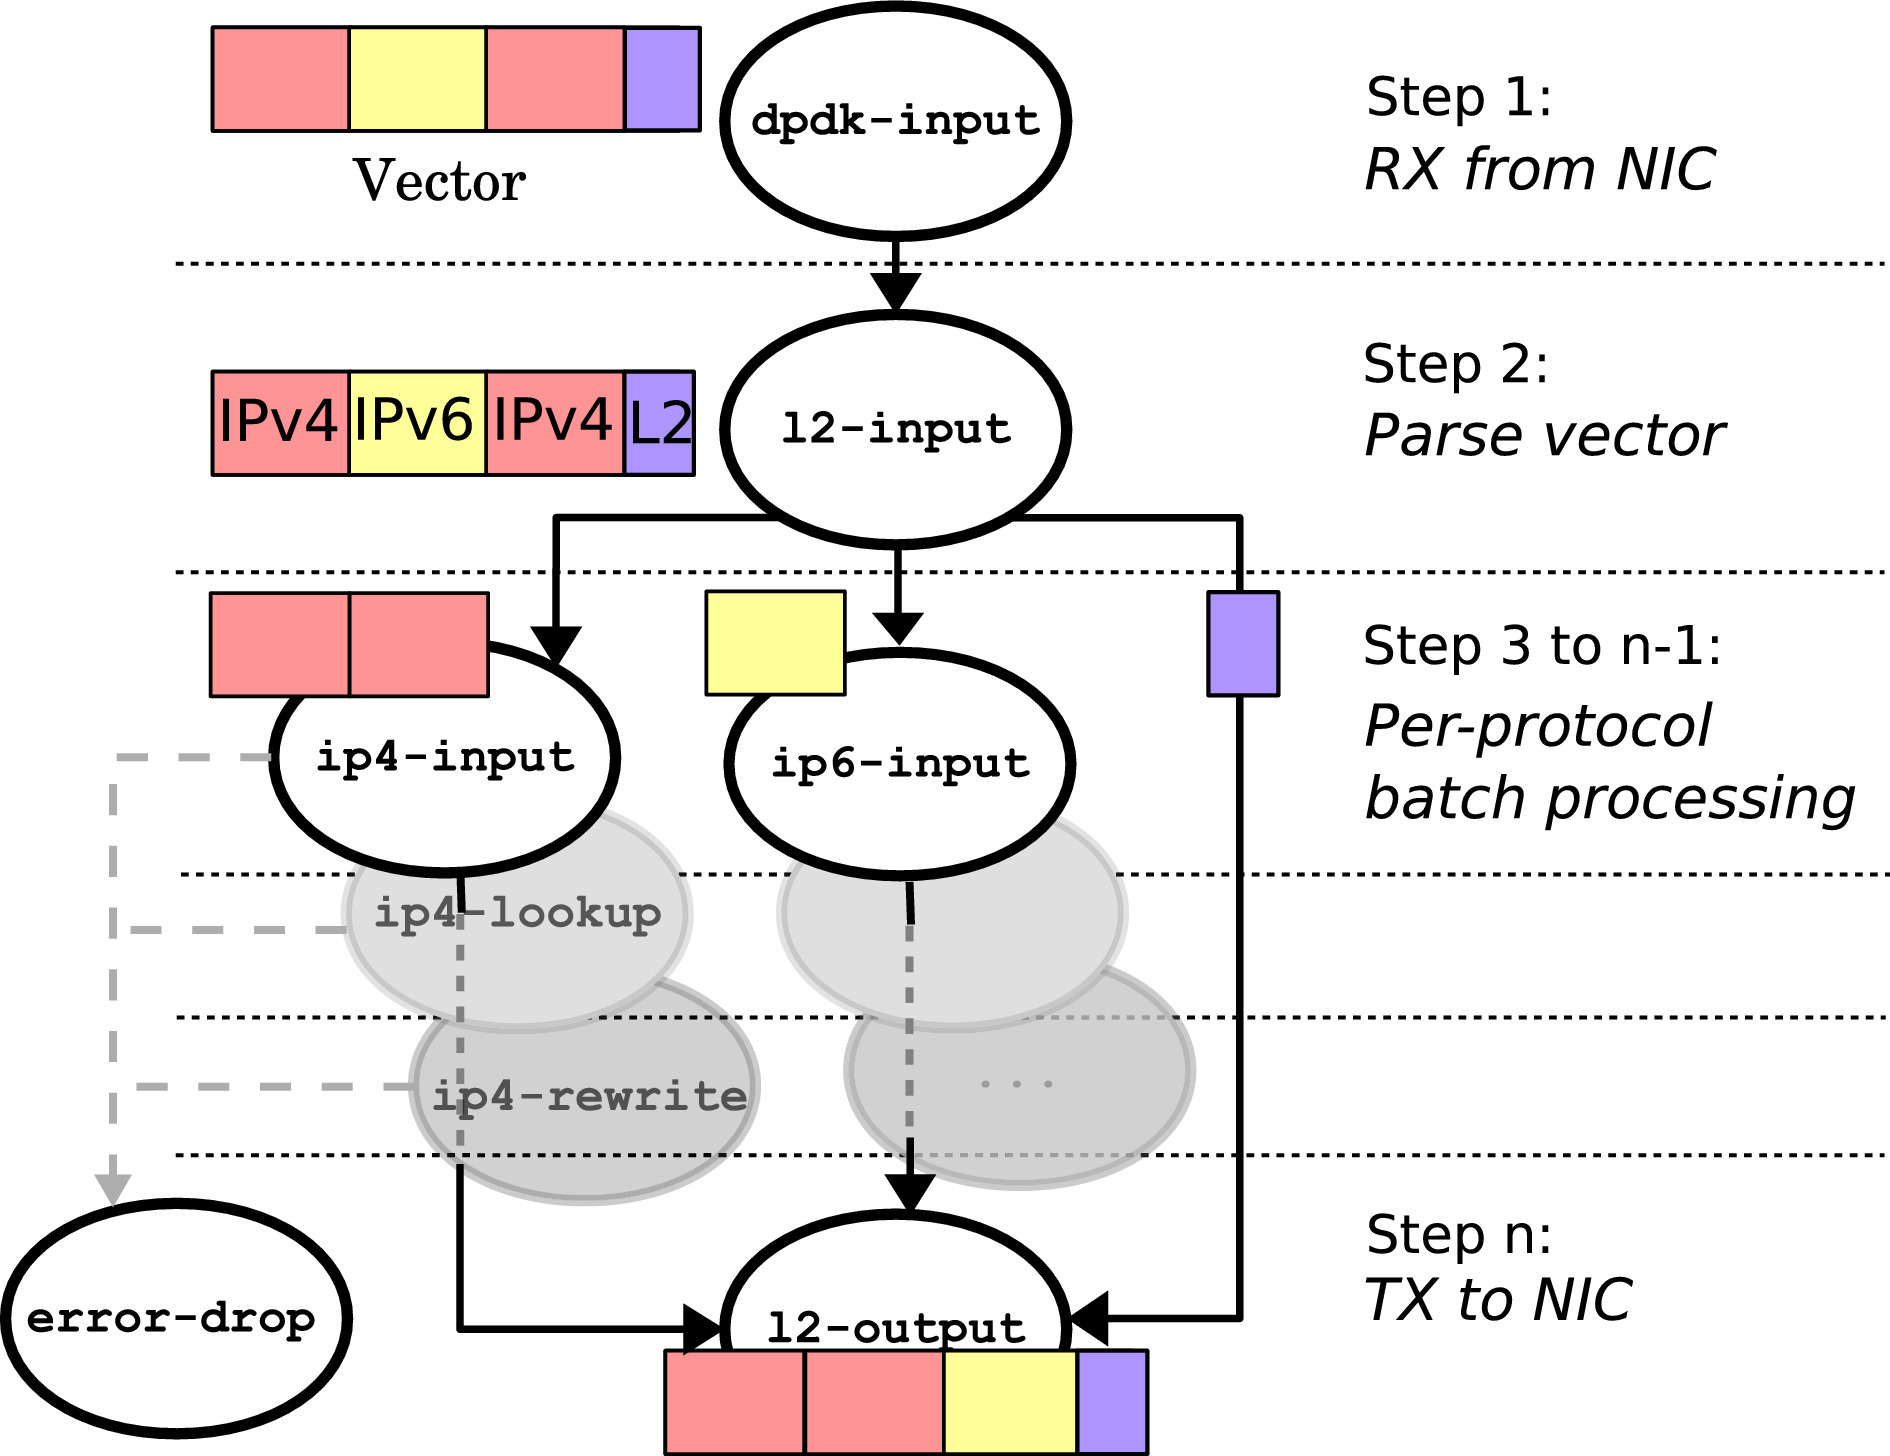
\includegraphics[width=0.7\linewidth]{images/processing-graph.jpg}
    \caption{Picture showing the VPP Processing Graph~\cite{LINGUAGLOSSA}}
    \label{fig:processing-graph}
\end{figure}

Thanks to VPP's modular design, the processing graph is highly customizable and extensible. 
New nodes -- referred to as plugins -- can be easily added to implement specific functionality or repleace existing ones. 
Plugins are shared libraries that are loaded during startup of VPP, and they are not dependent on the VPP source code, allowing them to be developed independently. 
Moreover, existing nodes can be rewired to modify the packet processing logic when necessary.\cite{LINGUAGLOSSA, DR:COMMAG-18, fdio_vpp_extensible_2021}

%--------------------------------------------------------------------
\subsection{DPDK and Its Role in VPP}
The Data Plane Development Kit (DPDK) is an open-source collection of libraries and drivers designed to support high-speed packet processing in user space. 
It was initially developed by Intel in 2010 and is now maintained as a Linux Foundation project. 
DPDK provides a set of APIs and components that allow applications to bypass the kernel network stack and directly access network interface cards (NICs) 
through poll-mode drivers (PMD), significantly reducing the overhead associated with traditional packet handling mechanisms.\cite{dpdk_about}

DPDK is used in VPP for interfacing with hardware. It is implemented as a plugin called \textit{dpdk-plugin}.\cite{LINGUAGLOSSA, DR:COMMAG-18} 

While VPP supports multiple mechanisms for accessing network devices, such as \textit{af\_packet}, to the best of the author's knowledge, DPDK is by far the most widely used option.

%--------------------------------------------------------------------
\subsubsection{Poll Mode Drivers}
Poll Mode Drivers (PMDs) are a key component of the DPDK framework. Unlike traditional network drivers, which rely on interrupts to signal packet arrival, 
PMDs continuously poll the network interface card (NIC) (specifically its RX queue) in a busy-loop, completely avoiding traditional interrupt-based mechanisms. 
This approach allows packets to be retrieved, processed, and delivered directly to user space without kernel involvement. 
While this results in very low latency and high throughput, it also causes constant CPU utilization on the cores assigned to polling, regardless of actual traffic load.\cite{FREITAS2022148}

Not every network interface card is supported by DPDK. Each supported device requires a specific Poll Mode Driver (PMD), which must be available and compatible with the given hardware. 
An up-to-date list of supported NICs and their corresponding PMDs is maintained on the official DPDK website.\cite{dpdk-supported-nics}

%--------------------------------------------------------------------
\subsubsection{Memory management and Hugepages}
DPDK uses a user-space memory model that eliminates the need for kernel involvement during packet processing. 
It operates on memory regions reserved as hugepages -- large memory pages, typically 2 MB or 1 GB in size, which are allocated at startup. 
These hugepages are used to store packet buffers and manage memory pools. 
DPDK defines its own memory management structures, such as mempools, which consist of preallocated fixed-size objects. 

DPDK is also explicitly NUMA-aware. Most memory allocation functions require the application to specify the target NUMA node, ensuring that memory is allocated close to the CPU core accessing it. 
This minimizes latency caused by cross-node memory access and helps optimize performance on multi-socket systems.\cite{burakov2019memory}

%--------------------------------------------------------------------
\subsubsection{Packet Reception and Transmission: A comparison between Linux Network Stack and DPDK}
When a packet arrives at a NIC managed by the Linux Network Stack, it is first stored in the NIC’s internal buffers. 
The NIC then writes the packet via Direct Memory Access (DMA) to the section of RAM provided by the driver and updates the corresponding descriptor in the RX buffer. 
The RX buffer is implemented as a ring queue.

Once the packet has been saved, the corresponding interrupt request (IRQ) is triggered to notify the CPU that one or more packets have arrived in that queue. 
Then, the corresponding IRQ handler is executed, which acknowledges the interrupt and calls the \textit{napi\_schedule} and \textit{\_\_raise\_softirq\_irqoff} functions.

The first function marks the associated \texttt{napi\_struct}%
\footnote{\texttt{napi\_struct} represents a NAPI context associated with a specific receive queue of a network device.}
 as ready for processing, while the second one raises a software interrupt (SoftIQR) specifically intended for processing incoming packets. 
Once the SoftIRQ is triggered, the kernel handles the actual packet processing in a deferred context. 
It goes through a list of network devices that have indicated pending work (i.e., their associated \texttt{napi\_struct} has been marked as ready) 
and calls their associated poll functions to retrieve and process packets from the receive queues.

This happens on the same CPU core that handled the original interrupt. If the system is busy or the processing takes too long, the remaining work may be handled by the \textit{ksoftirqd} kernel thread. 
The packets may be aggregated into a single larger packet using Generic Receive Offload (GRO), or processed individually. 
In both cases, they are passed to the IP stack via the \texttt{netif\_receive\_skb} function.

The transmission path is handled in a similar manner, using ring buffers, DMA, and deferred processing. 
However, unlike reception, packet transmission is initiated from the IP stack using the \texttt{\_\_dev\_queue\_xmit} function. 
Depending on the qdisc in use, packets are either enqueued in the software queue or passed directly to the driver for transmission.
Once a packet is selected for transmission, the driver places a descriptor into the TX ring buffer and sets up DMA so that the NIC can read the packet data from memory.
After the NIC finishes transmitting the packet, it triggers a TX interrupt, which allows the driver to perform post-processing such as unmapping DMA buffers and freeing memory.\cite{linux-packet-input}


When there is a NIC with multiple RX queues available, it is assigned to one of the queues based on the NIC's configuration%
\footnote{For network interface cards with multi-queue capabilities, the corresponding kernel driver often provides a module parameter to define how many hardware queues should be initialized and utilized.}.
The selection of the target queue is typically based on a hash function computed over network and/or transport layer headers.
Each queue has a dedicated IRQ, which can be assigned to specific CPU cores based on system settings. This mechanism is known as Receive Side Scaling (RSS).

When sending a packet from a NIC equipped with multiple TX queues, Transmit Packet Steering (XPS) is used to determine the appropriate TX queue.
The first option is that a CPU core is assigned specific TX queues. The second option is to use the TX queue corresponding to the RX queue from which the flow originated.
If multiple queues are eligible, a hash function is used to select the specific queue.\cite{linux-rss}

On the other hand, in DPDK the incoming packets are delivered by the network interface card (NIC) using direct memory access (DMA), 
which writes packet data into pre-allocated memory buffers specified by receive (Rx) descriptors.
These descriptors are organized in a circular ring (Rx queue), where the NIC populates entries at the head, while the VPP continuously polls the tail using functions such as                    
\textit{rte\_eth\_rx\_burst()}. This polling mechanism enables the VPP to retrieve multiple packets in a batch,
minimizing interrupt overhead and reducing latency, thereby increasing throughput and core efficiency.\cite{intel-core-utilization-2025}
 
Transmission is handled similarly, using a ring buffer known as the transmit (Tx) queue.
The application prepares transmit (Tx) descriptors at the tail of this queue, each containing the address and length of the packet to be sent.
These descriptors reference memory buffers (mbufs) holding the packet data. 
After the descriptors are written, the application updates the Tx queue’s tail pointer to notify the NIC that new packets are available.
The NIC then reads the descriptors from the head of the queue, fetches the packet data via DMA, and transmits the packets on the wire.\cite{intel-pcie-traffic-2025}

\begin{figure}[!htbp]
    \centering
    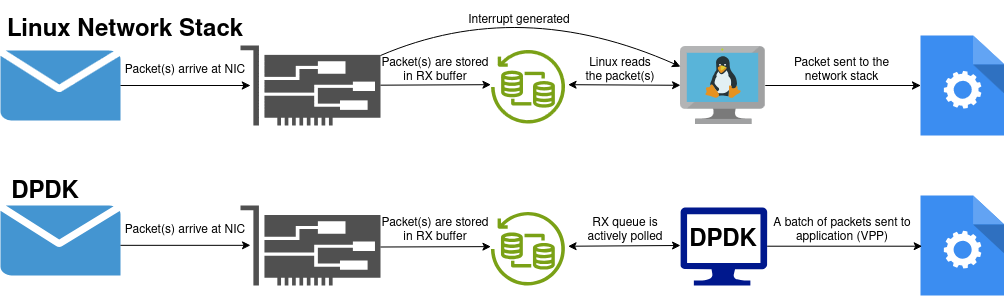
\includegraphics[width=0.99\linewidth]{images/dpdk-vs-linux.png}
    \caption{Diagram illustrating the differences in packet handling between the Linux Network Stack and DPDK.}
    \label{fig:dpdk}
\end{figure}

%COMPARISON
Based on the description above, several key differences between the Linux Network Stack and DPDK can be observed.
Although both rely on a similar underlying mechanism -- ring buffer queues -- their implementations differ fundamentally.
In the Linux Network Stack, memory management is handled by the kernel through device drivers. 
In contrast, DPDK allocates memory in user space and manages it through its own framework, providing packet buffers and ring structures directly to the application.

Linux is heavily dependent on hardware interrupts (IRQs) for packet reception and software interrupts (softIRQs) for deferred processing, which introduces frequent context switches. 
While NAPI uses polling to process packets from receive queues, they are still handled one at a time.
This increases the likelihood of cache misses during packet processing, as each packet is processed independently and may not benefit from cache locality.

In contrast, DPDK works entirely in user space and uses continuous active polling, completely bypassing the need for interrupts and context switching. 
Since it does not wait for an interrupt to occur, packet processing can begin sooner, reducing initial latency. 
Additionally, DPDK can retrieve multiple packets in a single burst, preparing them for vectorized processing in VPP.
Figure \ref{fig:dpdk} presents a simplified diagram highlighting the key differences.

%---------------------------------------------------------------
\section{Implementation of Vector Packet Processing}
%---------------------------------------------------------------
\subsection{DPDK and Its Role in VPP}

přesunout

The Data Plane Development Kit (DPDK) is an open-source collection of libraries and drivers designed to support high-speed packet processing in user space. 
It was initially developed by Intel in 2010 and is now maintained as a Linux Foundation project. 
DPDK provides a set of APIs and components that allow applications to bypass the kernel network stack and directly access network interface cards (NICs) 
through poll-mode drivers, significantly reducing the overhead associated with traditional packet handling mechanisms.\cite{dpdk_about}

The DPDK completely bypasses the kernel, communicating directly with the NIC.
DPDK avoids the use of the kernel’s system calls, instead handling its own I/O synchronization and memory management. 
DPDK employs a Poll Mode Driver (PMD) that uses busy-polling to retrieve, process, and deliver network packets to user-space applications without relying on interrupts. 
While this approach enhances performance by reducing latency, it also results in high CPU utilization, with the CPU usage on each core remaining close to 100\% regardless of the network load.\cite{FREITAS2022148}

DPDK is used in VPP for interfacing with hardware. It is implemented as a plugin called \textit{dpdk-plugin}.\cite{LINGUAGLOSSA, DR:COMMAG-18} 

%------------------------------------------
\subsection{VPP key architecture components}

VPP's dataplane is implemented by four main architectural layers: VPPINFRA, VNET, VLIB, and Plugins. 
Each layer provides distinct functionalities that support efficient networking operations, from low-level data structure management to high-level network function optimizations. 
The following sections describe these layers in detail: \footnote{https://my-vpp-docs.readthedocs.io/en/vpp-config/gettingstarted/developers/swarch/softwarearchitecture.html}

\begin{itemize}
  \item \textbf{VPPINFRA} -- layer providing foundational libraries for performing tasks with memory, vectors, rings, lookups in hash tables \& timers.
  \item \textbf{VNET} -- layer that deals with networking on layers 2 - 4 and is responsible for Control plane.
  \item \textbf{VLIB} -- layer that provides library for vector processing, implements CLI and handles application management functions.
  \item \textbf{Plugins} -- layer which is a set of plugins that allow for adding network functions and optimizations tailored to specific needs.
\end{itemize}

\subsubsection{VPPINFRA}
VPPINFRA is a collection of library services designed to offer high-performance capabilities for various tasks. 
It includes features such as dynamic arrays, hashes, bitmaps, high-precision real-time clock support, event logging, and data structure serialization. The following functionalities are implemented:

\begin{itemize}
  \item \textbf{Vectors} -- dynamically resized arrays with \textit{headers} defined by user. They serve as a core building block for other data structures (e.g., hash tables, pools) and allow efficient memory reuse via safe length resetting.
  \item \textbf{Bitmaps} -- dynamic bitmaps based on VPPINFRA vectors.
  \item \textbf{Pools} -- structures used to quickly allocate \& free fixed-size data structures. 
  \item \textbf{Hashes} -- structures thats provide fast key-value lookups, commonly mapping keys to indices in vectors or pools. Bihash is used in the data plane for fixed-size keys and is thread-safe, while the simpler hash is used in the control plane for exact string matching.
  \item \textbf{Timekeeping} -- service providing high-precision, low-cost timing based on CPU ticks. Since CPU ticks are not perfectly accurate, the system continuously adjusts its estimate of "ticks per second" by comparing with the kernel’s time. This results in precise and smooth time measurements without the need for expensive system calls. 
  \item \textbf{Timer wheel} -- system for efficiently managing timers or timeouts. It allows the user to define parameters like the number of wheels, slots per ring, and timers per object, optimizing time-based operations in systems requiring high-performance event management.
\end{itemize}

\subsubsection{VNET}
odmítám dělat teď

\subsubsection{VLIB}
Zítra je taky den

\subsubsection{Plugins}
Plugins are used to modify or create new features into the VPP. 
Developers can create plugins through a straightforward process, involving the generation of necessary files and integration into the build system. 
After building, the new plugin can be loaded and tested within the VPP environment. 

VLIB supports a simple mechanism for loading and using plugins. 
VLIB client applications specify a directory where the plug-ins are located and can apply a filter to narrow down the search. 
Once the plug-ins are loaded, VLIB ensures they are correctly registered and ready for use.


%--------------------------------------
\subsection{Configuration and Startup}



%---------------------------------------------------------------
\chapter{Pratical part}
%---------------------------------------------------------------

%---------------------------------------------------------------
\section{Building Infrastructure for Measurement}
%---------------------------------------------------------------

%---------------------------------------------------------------
\section{Test Scenarios \& Results}
%---------------------------------------------------------------

%---------------------------------------------------------------
\subsection{Scenario \#1a}
%---------------------------------------------------------------

%---------------------------------------------------------------
\section{Presentation and Analysis of Results}
%---------------------------------------------------------------



